\chapter{Introduction}

%%The merger of two white dwarfs (WDs) originally in a short-period binary is estimated (eg. \citealt{badem12}) to occur about once every century in a Milky Way-like galaxy, making the products of such events common throughout the universe.  They have been held responsible for producing a variety of stars with strange properties, including helium-burning sdOB stars \citep{saioj00, justph11}, RCrB stars (eg. \citealt{webb84, clay+07, clay13}), and massive and highly magnetized WDs (eg. \citealt{segrcm97, garc+12, kule+13}) that could resemble the hot DQ WDs (eg. \citealt{dunlc15}, Dunlap and Clements in preparation).  They may, however, also be responsible for spectacular transient events including accretion-induced collapses (eg. \citealt{saion85, abdi+10}) and type Ia supernovae (SNe Ia; eg. \citealt{howe11, hill+13, maozmn14}).  Determining the final outcome of a particular merger requires an understanding of the detailed dynamics of the merging process, which cannot directly be seen using current observational capabilities.  Thus, studies of merger physics have primarily utilized hydrodynamic simulations.

\section{The Panopoly of Stellar Mergers}
\label{sec:c1_stellarmergers}

Approximately two out of every three stars are born into a binary system.  A substantial fraction of these stars will interact, some due to their orbital separation at birth, while others following the expansion of one or both constituent stars as they evolve off of the main sequence.  These interactions primarily take form as mass transfer between the stars \citep{yung05}, and if mass transfer becomes unstable (increases exponentially over time), it ends with the violent coalescence of the two stars into one.  These stellar mergers, like other forms of binary interaction, disrupt single star evolution and create merged products, or ``merger remnants'', with unusual properties including blue stragglers (eg. \citealt{andrpt06, knigs09}), luminous blue variables \citep{justpv14}, subdwarf OB and R Coronae Borealis stars.

Mergers also liberate tremendous amounts of energy and eject significant amounts of mass, giving rise to a cornucopia of electromagnetic (and gravitational-wave) transients ranging from luminous red novae (from the merger of two (post-) main-sequence stars; eg. V838 Monocerotis and V1309 Scorpii \citep{tyle+11, nandil14}) to short gamma-ray bursts (from two neutron stars; eg. \citealt{ross15}) and the gravitational wave outburst from coalescing stellar-mass black holes (as recently found by the LIGO detector; \citealt{ligo16}).  Indeed, with current deep and short-cadence optical/near-infrared survey projects such as the Palomar Transient Factory \citep{rau+09} and Pan-STARRS \citep{kais+10} continuing to uncover more rare and even hitherto-unknown transients, and the ambitious Large Synoptic Survey Telescope \citep{lsst09} under construction, a much more complete picture of merger-generated transients will form over the next decade.

% Sec 5.2.3 of Tylenda talks about MS - MS pre-merger orbital evolution.

\section{Mergers of Two White Dwarfs}
\label{sec:c1_wdmergers}

Stars with masses $\lesssim8-10\,\Msun$ generally end their lives as white dwarfs (WDs).  On their own, WDs are usually inert: held up against gravity by electron degeneracy pressure (eg. \cite{kippww12}, Ch. 15) and having ceased nuclear fusion, they will slowly radiate away their remaining thermal energy over billions of years if left alone.  WDs in interacting binaries, on the other hand, can receive mass and energy from their stellar companion, leading to a whole host of energetic and potentially explosive phenomena.

\subsubsection{The Formation of Double White Dwarf Binaries}

One common end-product of binary evolution is a pair of white dwarf (WDs).    These binaries are formed as a result of at least two phases of mass transfer (at least one of which is a common envelope event) during the binary's prior stellar evolution.  These mass transfer phases act to sap the orbital angular momentum of the 

%http://adsabs.harvard.edu/abs/2008MNRAS.387.1693C

%(Weidemann 2000, A&A 363, 647;
%Catalan et al. 2008, MNRAS 387, 1693)
%Toonen and Mennekens pop synth codes

\begin{figure}
\centering
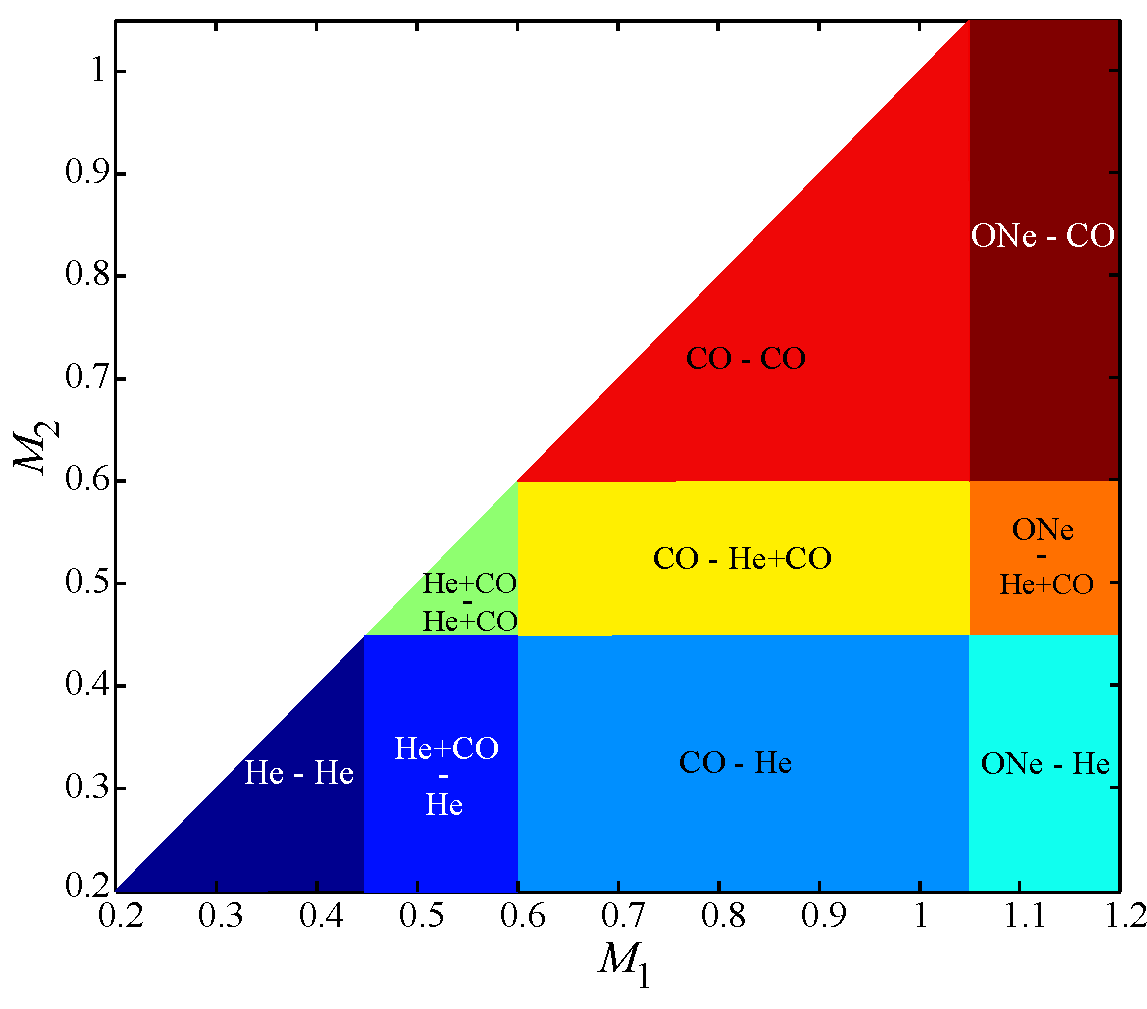
\includegraphics[width=0.6\hsize]{introduction/figures/dan+12_wdbinmass.pdf}
\caption{The mass parameter space of double WD binaries, subdivided by the dominant chemical compositions of the WDs, from \cite{dan+12}, their Fig. 1.  $M_1$ is the mass of the primary, or accreting, WD, and $M_2$ is the mass of the secondary, which donates mass.  WDs with masses $M<0.45\,\Msun$ are assumed to be He WDs, those with $0.45 < M < 0.6\,\Msun$ CO WDs with $\sim0.1\,\Msun$ He envelopes, $0.6 < M < 1.05\,\Msun$ CO WDs, and $M>1.05\,\Msun$ ONe WDs.  See text, as well as \cite{dan+12}, Sec. 2, for discussion on these choices.}
\label{fig:c1_wdbinarymasses}
\end{figure}

The mass and composition of each WD within the binary are dependent on the binary's prior evolution, and therefore are related to one another.  Broadly speaking, WDs with masses $M \lesssim 0.45\,\Msun$ are composed of helium (He), since these come from stars that had their evolution interrupted by binary interaction while on the RGB (eg. \citealt{marsdd95, nele+01, nele+01a}), before their degenerate He core became massive enough to trigger a helium flash (eg. \cite{kippww12}, Ch. 33.4).  (They could in principle also come from single stars of $\lesssim0.5\,\Msun$, but the universe is not old for any He WD to have been born this way {\charles CITATION}.)  WDs with slightly higher masses have He envelopes surrounding cores composed of carbon and oxygen (CO); \cite{dan+12} approximate the mass range of these ``hybrid WDs'' to be $0.45 \lesssim M \lesssim 0.6\,\Msun$.  From $0.6 \lesssim M \lesssim 1.1\,\Msun$ WDs are almost entirely composed of CO, with He atmospheres of $\sim10^{-2}\,\Msun$ (eg. \citealt{ibent85}).  WDs with masses $\gtrsim 1.1\,\Msun$ come from super-AGB stars (eg. \citealt{herw05}) that ignite carbon during their evolution (eg. \citealt{garc13}), and thus are composed at least partly of oxygen and neon (ONe).  

Fig. \ref{fig:c1_wdbinarymasses}, from \cite{dan+12}, summarizes these relationships for the WD binary parameter space -- in it, $M_1$ is the mass of the (more massive) primary WD, which accretes mass during the merger, and $M_2$ is the mass of the secondary, which donates mass (Sec. \ref{ssec:c1_stable_mass_transfer}).  While nature is not so clear-cut (eg. \citealt{ibent85, moros09} for CO WDs with $M\lesssim0.45\,\Msun$ and \citealt{hurlpt00} for CO WDs with $M\gtrsim1.2\,\Msun$), these relationships are used as rules of thumb for setting WD composition for a wide range of works (\citealt{loreig09,rask+12,dan+12,dan+14}, with slight variations between different research groups) for setting the composition).  In this thesis, we generate binaries of CO WDs with masses ranging from $0.4 - 1.0\,\Msun$ for our parameter space study of mergers in Ch. \ref{ch:ch2}.  In subsequent chapters, we are primarily interested in the the merger of two CO WDs near the median mass of field WDs, $\sim0.65\,\Msun$ (Sec. \ref{ssec:c1_cowd_massrange}).

The ratio of carbon and oxygen within CO WDs is also not particularly well-known.  In this thesis, we make the assumption that they are composed of 50\% carbon and 50\% oxygen by mass.  {\charles ADD STUFF}

\subsubsection{Orbital Angular Momentum Loss and Gravitational Wave Emission}

Following their formation, these binaries can lose orbital angular momentum through a number of of mechanisms, including gravitational radiation (eg. \citealt{petem63}), magnetic braking (eg. \citealt{verb84}) or the influence of a third body (eg. \citealt{katzd12}).  {\charles TIDAL EFFECTS?}  In the absence of a magnetized wind or third body, gravitational radiation is generally thought to be the dominant driver of angular momentum loss, and has a characteristic timescale of \citep{segrcm97}

\eqbegin
\tau_{\mrm{grav}} = 5 \times 10^5 \left(\frac{a}{10^5 \mrm{km}}\right)^4 \frac{\Msun}{\Ma} \frac{\Msun}{\Md} \frac{\Msun}{\Mtot}\,\mrm{yr}.
\label{eq:c1_gravtimescale}
\eqend

\noindent From this, we see that WD binaries with orbital periods on the order of hours or less will merge within a Hubble time.  It is estimated that there are on order of $10^8$ such systems in the Milky Way alone \citep{mars11}.

While inspiralling WD binaries with periods on the order of minutes are too low-frequency to be detected by Advanced LIGO (Laser Interferometer Gravitational-Wave Observatory \citealt{ligo+15}), they are expected to be the most numerous and dominant source of gravitational waves \citep{mars11} detected by the proposed spaceborne detector eLISA (evolved Laser Interferometer Space Antenna; \citealt{amar+13}), which probes the mHz frequency range.  Individual signals from thousands of WD binaries that are $\sim1\,\mrm{Myr}$ prior to merger can be individually resolved with eLISA \citep{amar+13,loreig09, dan+11}, while the numerous sources further away and at at longer orbital periods (lower frequencies) will comprised an unresolved background \cite{neleyp01,amar+13}.  Both of these will probe the WD binary population of the Milky Way without the selection biases that often trouble electromagnetic binary searches \citep{mars11}.  {\charles Note, however, that final coalescence of the WDs is over far too quickly to be detectable by eLISA.}  The energy lost to gravitational radiation also plays a negligible role during the merger, being is $\sim10^{-10}$ of the binary's binding energy (eg. \citealt{loreig09}).

\subsubsection{Merger Outcomes}

Like any merger, those between WDs liberate tremendous amounts of energy.  This can lead to enough heating and/or compression to reignite the nuclear furnaces of normally inert WDs under either non-degenerate or degenerate circumstances.  As such, the end product of such mergers are diverse, ranging from stars with unusual properties undergoing stable nuclear burning to explosions. Hydrostatic (and non-rotating, unmagnetized {\charles CITATION}) WDs have a maximum stable mass beyond which bodies supported by electron degeneracy pressure are unstable to collapse.  This is known as the \cite{chan31} mass, or \Mch, and is at $\sim1.4\,\Msun$.  This has long led to the notion that sufficiently massive WD mergers can lead to the complete destruction of the merger product, either in a thermonuclear explosion that would resemble type Ia supernovae (SNe Ia; \citealt{webb84}), or transformation into a neutron star (NS) in an event known as an accretion-induced collapse \citep{nomoi85, saion85}.  Today, however, we know of a much greater range of possible merger outcomes, both for binary systems with masses above and below \Mch.  Which outcome occurs depends largely on the compositions of the WDs involved, and are briefly summarized below (see also \citealt{dan+14}, who produce a similar list):

% dan+14 Fig 12, dan+12 fig 8

\begin{itemize}
	\item The merger of {\bf two He WDs} is unlikely to lead to violent nuclear burning and an explosion \citep{dan+12,dan+14,dan+15}.  Instead, merger remnants with total masses $0.4\lesssim \Mtot \lesssim 0.8$ \citep{han+02,pacz71}\footnote{This is lower than the He flash mass of $\sim0.45\,\Msun$ because the merger remnant is partly non-degenerate \citep{han+02}.}, which are the vast majority of double He WD remnants \citep{nele10}, are expected to ignite He burning in a shell \citep{saioj00,zhanj12}.  This increases the radius and luminosity of the star until it becomes a yellow giant after $\sim 10^3-10^4\,\mrm{yr}$, with properties similar to Extreme Helium (EHe) and R Coronae Borealis (R CrB) stars {\charles \citep{saioj00, zhanj12}.}  Over the next $10^5-10^6\mrm{yr}$, the burning shell migrates inward with a series of weakening shell flashes, while the radius slowly shrinks to $\sim10^{-1}\,\Rsun$.  Once the shell reaches the center of the remnant, stable He fusion is ignited, and remnant settles onto the helium main sequence, resembling a subdwarf B (sdB) or O (sdO) star \citep{saioj00, justph11, zhanj12}.  While most subdwarf stars are in binaries, and likely form from other formation channels channels, mergers are expected to be a major -- perhaps even the main -- source of single subdwarf stars (eg. \citealt{han+03, nele10}).

	\item The outcome of a merger between {\bf an He and a CO WD}, or a merger between an He and hybrid He-CO WD, depends on whether or not a He explosion is touched off during the merger.  Roughly speaking, mergers with $\Mtot \lesssim 0.8\,\Msun$ are unlikely to trigger an explosion \citep{dan+12, dan+14} and will instead ignite He burning in a shell; they have been proposed as the progenitors to He-rich sdO stars (\citealt{justph11}; He-poor sdO stars are likely evolved sdB stars).  Mergers with $\Mtot \gtrsim 0.8\,\Msun$ that do not experience an explosion will also ignite shell burning, but unlike sdOB progenitors they will retain their extended envelope for the duration of their burning phase \citep{pacz71}.  These mergers are believed to be the primary formation channel for Hydrogen-deficient Carbon (HdC) and R CrB stars \citep{webb84, ibent84, saioj02, clay12, kararh15}, which are H-deficient, He- and C-rich supergiants that, in the case of R CrB stars, feature abrupt variability by up to a factor of $\sim10^3$ due to the formation of carbon dust above their photospheres.  Following He shell exhaustion, they will contract in radius and heat up their envelopes, becoming consistent with EHe stars \cite{saioj02, jeff14}.

Helium explosions become more likely for binaries with $\Mtot\gtrsim\Mch$ \citep{dan+12, dan+14}.  In cases where an accreted He shell explodes, but the underlying CO WD remains, the result depends on a number of factors including the mass of the CO WD and amount of He it accretes, and spans a wide range of possible peak luminosities \citep{woosk11}.  Detonations (or deflagrations; \citealt{wooswk11}) of $\lesssim0.1\,\Msun$ He shells lead to explosions that reach peak brightnesses of factors of $\sim10-100$ lower than SNe Ia, in $\sim2-10$ days (typical SNe Ia values are in Sec. \ref{sec:c1_mysteryofsneia}), making them similar to the ``.Ia SNe'' theorized to occur in AM Canum Venaticorum binaries \citep{bild+07}.  They synthesize Ca, Cr and Ti, but relatively little of the radioactive \Ni\ typically seen in SNe Ia \citep{shen+10he, woosk11, wald+11}.  Denser He envelopes (due to it or the CO WD accretor being more massive), tend to synthesize more \Ni\ in detonations \citep{shen+10he, wald+11}. 

\cite{wald+11} also suggest that the detonation of $\sim0.2\,\Msun$ of He on top of a $\sim0.45\,\Msun$ CO WD could explain the SN 2005E-like class \citep{pere+10} of low-luminosity SNe Ib that produce very little \Ni, have low ejecta masses and spectroscopically show strong lines of He, Ca and Ti.  While these masses are remarkably low, \cite{shen+10he} and \cite{wald+11} model thick hydrostatic He envelopes around CO cores, and these will be much denser than He envelopes in merger remnants.

% moreover simulations suggest He detonations in mergers occur before an He envelope of more than a few $10^{-2}\,\Msun$ can accrete onto the disk.

%Less degenerate material will lead to explosions dominated by lighter elements like Ca \citep{woosk11}, and therefore He detonation may be possible in really massive systems.  Dan+14 already had that idea though; see below.

In the case where the the He shell detonates, and triggers the CO WD to do the same -- a ``double-detonation'' -- an SN Ia may be produced (Sec. \ref{ssec:c1_new_typeia}).

	\item The merger of {\bf two CO WDs} has long been suspected of producing an SN Ia under the right conditions (Sec. \ref{sec:c1_mysteryofsneia} and \ref{sec:c1_vkchannel}).  If these conditions are not met, they will instead create a lone massive, rotating and highly magnetized CO WDs or, if steady carbon fusion is ignited, a carbon-burning star that eventually turns into an ONe WD (Sec. \ref{sec:c1_hotdqs}).  If the ONe WD is above \Mch, it may experience an AIC (see below).

	\item Due to their mass, it is likely that the merger of {\bf an ONe WD} with any companion will create a super-\Mch\ remnant.  Unlike their CO counterparts, ONe WDs that are compressed through accretion to $\gtrsim3\times10^9\,\gcc$ initiates electron-capture reactions onto $^{20}$Ne and $^{24}$Mg, losing degeneracy support in the process (eg. \citealt{miya+80, saion85, schwqb15}).  This leads it to further contract, likely\footnote{Since the electron capture reactions are exothermic, they trigger a thermal runaway that eventually starts an O-deflagration at $\sim10^{10}\,\gcc$.  Whether or not collapse or explosion occurs depends on exactly when the deflagration ignites; see, eg., discussion in \cite{schwqb15}.} experiencing an ``accretion-induced collapse'' (AIC) into a neutron star soon after its central density reaches $\sim10^{10}\,\gcc$ \citep{schwqb15}.  Simulations \citep{dess+06, dess+07, frye+09} of the AIC find it expels only $\sim10^{-2}\,\Msun$ of material and produces negligible amounts of radioactive \Ni, suggesting a very faint transient.

%Note - oxygen pycnonuclear fusion occurs well beyond 10^10 gcc (Fig. 12 Schw+15)

\cite{dan+14} discusses the possibility that He - ONe and CO - ONe WD mergers will lead to enshrouded AIC that produce ``hybrid supernovae'', where much of the outer envelope (of a different composition) explodes rather than collapsing.  They suggest in particular that a significantly super-\Mch\ He - ONe merger could lead to a He detonation resembling the SN 2005E-like SNe Ib discussed earlier.

\cite{marq+15} suggest that an ONe WD could be detonated, perhaps from the same double-detonation and violent merger mechanisms that could cause CO WDs to detonate (Sec. \ref{ssec:c1_new_typeia}).  Due to their high densities, these would tend to produce $\gtrsim1\,\Msun$ of \Ni, but, because fusing to \Ni\ from O and Ne generates $\sim30$\% less energy than from C \citep{marq+15}, also weaker explosions.  Detonations during ONe mergers may explain supernovae such as SN 2009dc \citep{taub+09} that are a factor of $\sim3$ brighter than SNe Ia at peak light, decay by a factor of $\sim3$ more slowly slower after peak light, and low expansion velocities.

\end{itemize}

Of these possibilities, those mergers that are theorized to create SNe Ia are particularly intriguing, as they may hold the key to solving the long-standing SN Ia progenitor problem.
